\BiChapter{统计分布}{}
	\BiSection{一点想法}{}
		私以为, 我们在学习一个东西的时候主要是要发现其中的动机(Motivation). 对于前人如何提出这个问题的, 尤其要关注. 而且, 对于书本上的逻辑, 看似是严谨的, 但是, 经常为了严谨, 而丢掉了发现的过程, 这个就少了很多乐趣了. 而且, 最让人感到不满意的一点, 许多结论的组织, 显得极为突然. 让人没有一个比较明晰的脉络. 所以, 这一章主要从三大统计分布中的$\chi^2$ 和 $t$ 分布的历史出发给出一点不一样的讲述.
		
	\section{$\chi^2$分布}
		\subsection{历史}
			麦克斯韦(Maxwell)在推导气体分子的运动的时候给出了一个衡量气体分子速率的公式. 称之为麦克斯韦速率分布函数:
			\begin{equation}
				f(v) = 4 \pi \left(\frac{m}{2\pi kT} \right)^{3/2} v^2 e^{-\frac{mv^2}{2kT}}
			\end{equation}
			且
			\begin{equation}
				\int_0^\infty f(v) dv = 1
			\end{equation}
			
			由于气体速度在各个方向上的投影速率服从正态分布, 从而, 速度的模方应该服从自由度为 3 的卡方分布. 那么, 我们可以来看一看, 在上面这个式子中, 在保证归一化条件的情况下做一个变换, 得到:
			
			\begin{equation}
				f(v^2) = 2 \pi \left(\frac{m}{2\pi kT} \right)^{3/2} \sqrt{v^2} e^{-\frac{mv^2}{2kT}}
			\end{equation}
	
			这是因为 $dv^2 = 2vdv$. 不难发现这该公式和卡方分布的相似性.
			
			这个分布还在其他的一些地方导出过.
		\subsection{$\chi^2$检验的另外一个小故事}
			当年威尔登(Weldon)做了一个实验, 把 12 个 6 面色子投掷了 26306 次, 每次记录下其中 5 或 6 出现的次数.
			
				\begin{table}[h]
					\centering
					\begin{tabular}[c]{crr}
						\toprule[1.5pt]
  						出现5或6的次数 & 观测值 & 理论值\\
						\midrule[1.5pt]
					    0 & 185 & 203 \\
						1 & 1149 & 1217 \\
						2 & 3265 & 3345 \\
						3 & 5475 & 5576 \\
						4 & 6114 & 6273 \\
						5 & 5194 & 5018 \\
						6 & 3067 & 2927 \\
						7 & 1331 & 1254 \\
						8 & 403 & 392 \\
						9 & 105 & 87 \\
						10 & 14 & 13 \\
						11 & 4 & 1 \\
						12 & 0 & 0 \\
						\bottomrule[1.5pt]
					\end{tabular}
					\caption{26306次投掷的实验结果}
				\end{table}

			
			但是, 皮尔逊观察了整理出来 的结果后, 认为色子可能有问题.	他的理由是这个样子的, 他发现其中 ``4" 这一组出现的次数为 $6114$ 次, 但是, 实际上的理论值是 $26306 \cdot C_{12}^4 (\frac{1}{3})^4(\frac{2}{3})^8 \approx 6273$ 次. 
			
			不妨来做一个计算. 设随机变量$Y$表示在一次投掷中出现5或6的个数恰为4. 那么 $Y \sim B(p, 1)$, $p = C_{12}^4 (\frac{1}{3})^4(\frac{2}{3})^8 \approx 0.238446$, 我们要投掷 $26306$ 次, 这个样本的数量足够大, 所以可以用正态分布去逼近这个二项分布, 可以得到这个二项分布的标准差为 $\sigma =\sqrt{np(1-p)} \approx  69.1151 $, 这时, 我们发现出现的次数和所估计的值差了$2.3\sigma$ 左右, 这个显然是一个比较大的偏差. 但是, 两位学者在讨论的时候也觉得这个极端的例子有些不妥, 还是应该从整体上去考虑.
			
			所以, 皮尔逊在 1900 年证明了一个定理. 
			\begin{theorem}
				设一个总体$X$服从某个分布, 作为一个假设, 认为$X$的分布为:
				\begin{equation}
					H_0: P(X_i = a_i) = p_i, i = 1, 2, \cdots, k
				\end{equation}
				
				那么, 从整体中进行 $n$ 次抽样, 其中 $X_i$ 的观测值为 $\nu_i$, 那么 统计量 
				\begin{equation}					
					Z = \sum_{i=1}^{k} \frac{(np_i - \nu_i)^2}{np_i} \sim \chi^2_{k-1}
				\end{equation}
			\end{theorem}
			
			经过计算, 可以得知上面这个问题的$Z = 43.87241$, 查$\chi^2$ 分布表可以知道, $\alpha\approx 0.000016$. 这个是奇怪的结果. 它告诉我们假设色子均匀的假设被拒绝了. 但是, 一个同样有趣的事情是, 皮尔逊在威尔登的建议下使用色子的实际投出四次5或6的频率$0.3377$去估计的时候, 得到的结果是$Z = 17.77576$, 此时, $\alpha \approx 0.1227$ 所以, 比较有把握说这个色子有大概 $10^{-3}$ 的偏差.
			但是, 这个偏差已经非常小了. 所以, 这个色子的均匀度已经足够了. 所以, 我们不能生搬硬套统计计算得到的结果. 
			
			 
	\section{$t$ 分布}
		哥塞特(Gosset)提出$t$分布的最初的想法, 其实, 不是从这个分布的定义来的. 而是他在开创小样本的计算理论的时候所研究的一个现实的问题. 所谓的小样本, 就是对于一个统计方法,如果它在定义中未涉及要求样本量$n\rightarrow \infty$那么就称这个方法是小样本的. 哥塞特的研究, 就是要把这个大和小的分界找到.
		
		\subsection{对$t$分布的研究}
			哥塞特认为: 如果样本量比较大, 那么认为$\frac{\bar{x}}{s}$是正态分布是可信的.
			但是如何才能导出这个东西的分布, 哥塞特并不是推出来的, 而是猜出来的, 他猜出了$s^2$的分布, 同时又证明了样本均值与样本方差不无关. 然后再计算出这两个随机变量商的分布.
			
			我们在这个地方介绍一个比较简单的证明他们之间的独立性的方法, 这个方法是由费舍尔(Fisher)最早提出的. 
		\subsection{$n$ 维几何法}
			费舍尔的$n$维几何法就是把样本$(x_1, x_2, \cdots, x_n)$ 看作 $n$ 维欧氏空间$R^n$中的点. 一个点落在一个微元区域的概率就是分布的概率元. 在这个问题中, 对于$\bar{x}$ 与 $s$ 的联合分布(设总体的均值为 0), 则要设法计算出点落入			
			\begin{equation} \label{ndgeometry}
				\{(x_1, x_2, \cdots, x_n): \xi_0 \le \xi_0 + \Delta \xi, \eta_0 \le \eta \le \eta_0 + \Delta \eta_0 \}
			\end{equation} 的概率.
			
			在这个地方.
			\begin{equation}
				\xi = \sqrt{n} \bar{x}
			\end{equation}
			
			\begin{equation}
				\eta = \sqrt{\sum_{i=1}^n (x_i - \bar{x})^2}
			\end{equation}
			
			这两个定义和前面所述的 $\bar{x}$ 和 $s$ 只有系数上的不同. 之所以要这么改变, 是为了几何上的方便. 比如说这个地方的 $\eta$ 是一个欧氏距离的表达式的形式. 
			
			那么, 对于一次抽样所得的样本, 我们可以计算出这个样本的均值, 定义点 $\xi_0 = (\bar{x}, \bar{x}, \cdots, \bar{x})$ 并把它画在 $R^n$中, 不难发现, 在给定样本方差的情况下, 样本点和这个均值点之间的距离是不变的, 所以它为于一个超球面上, 同时也不难发现, 样本点到均值点的向量和均值点到原点的向量之间是垂直的(可以由这两个相量的点积直接得到验证), 所以, 这个样本点位于一个低两维的空间内的球面上. 
			
			\begin{figure}[h]
				\centering				
				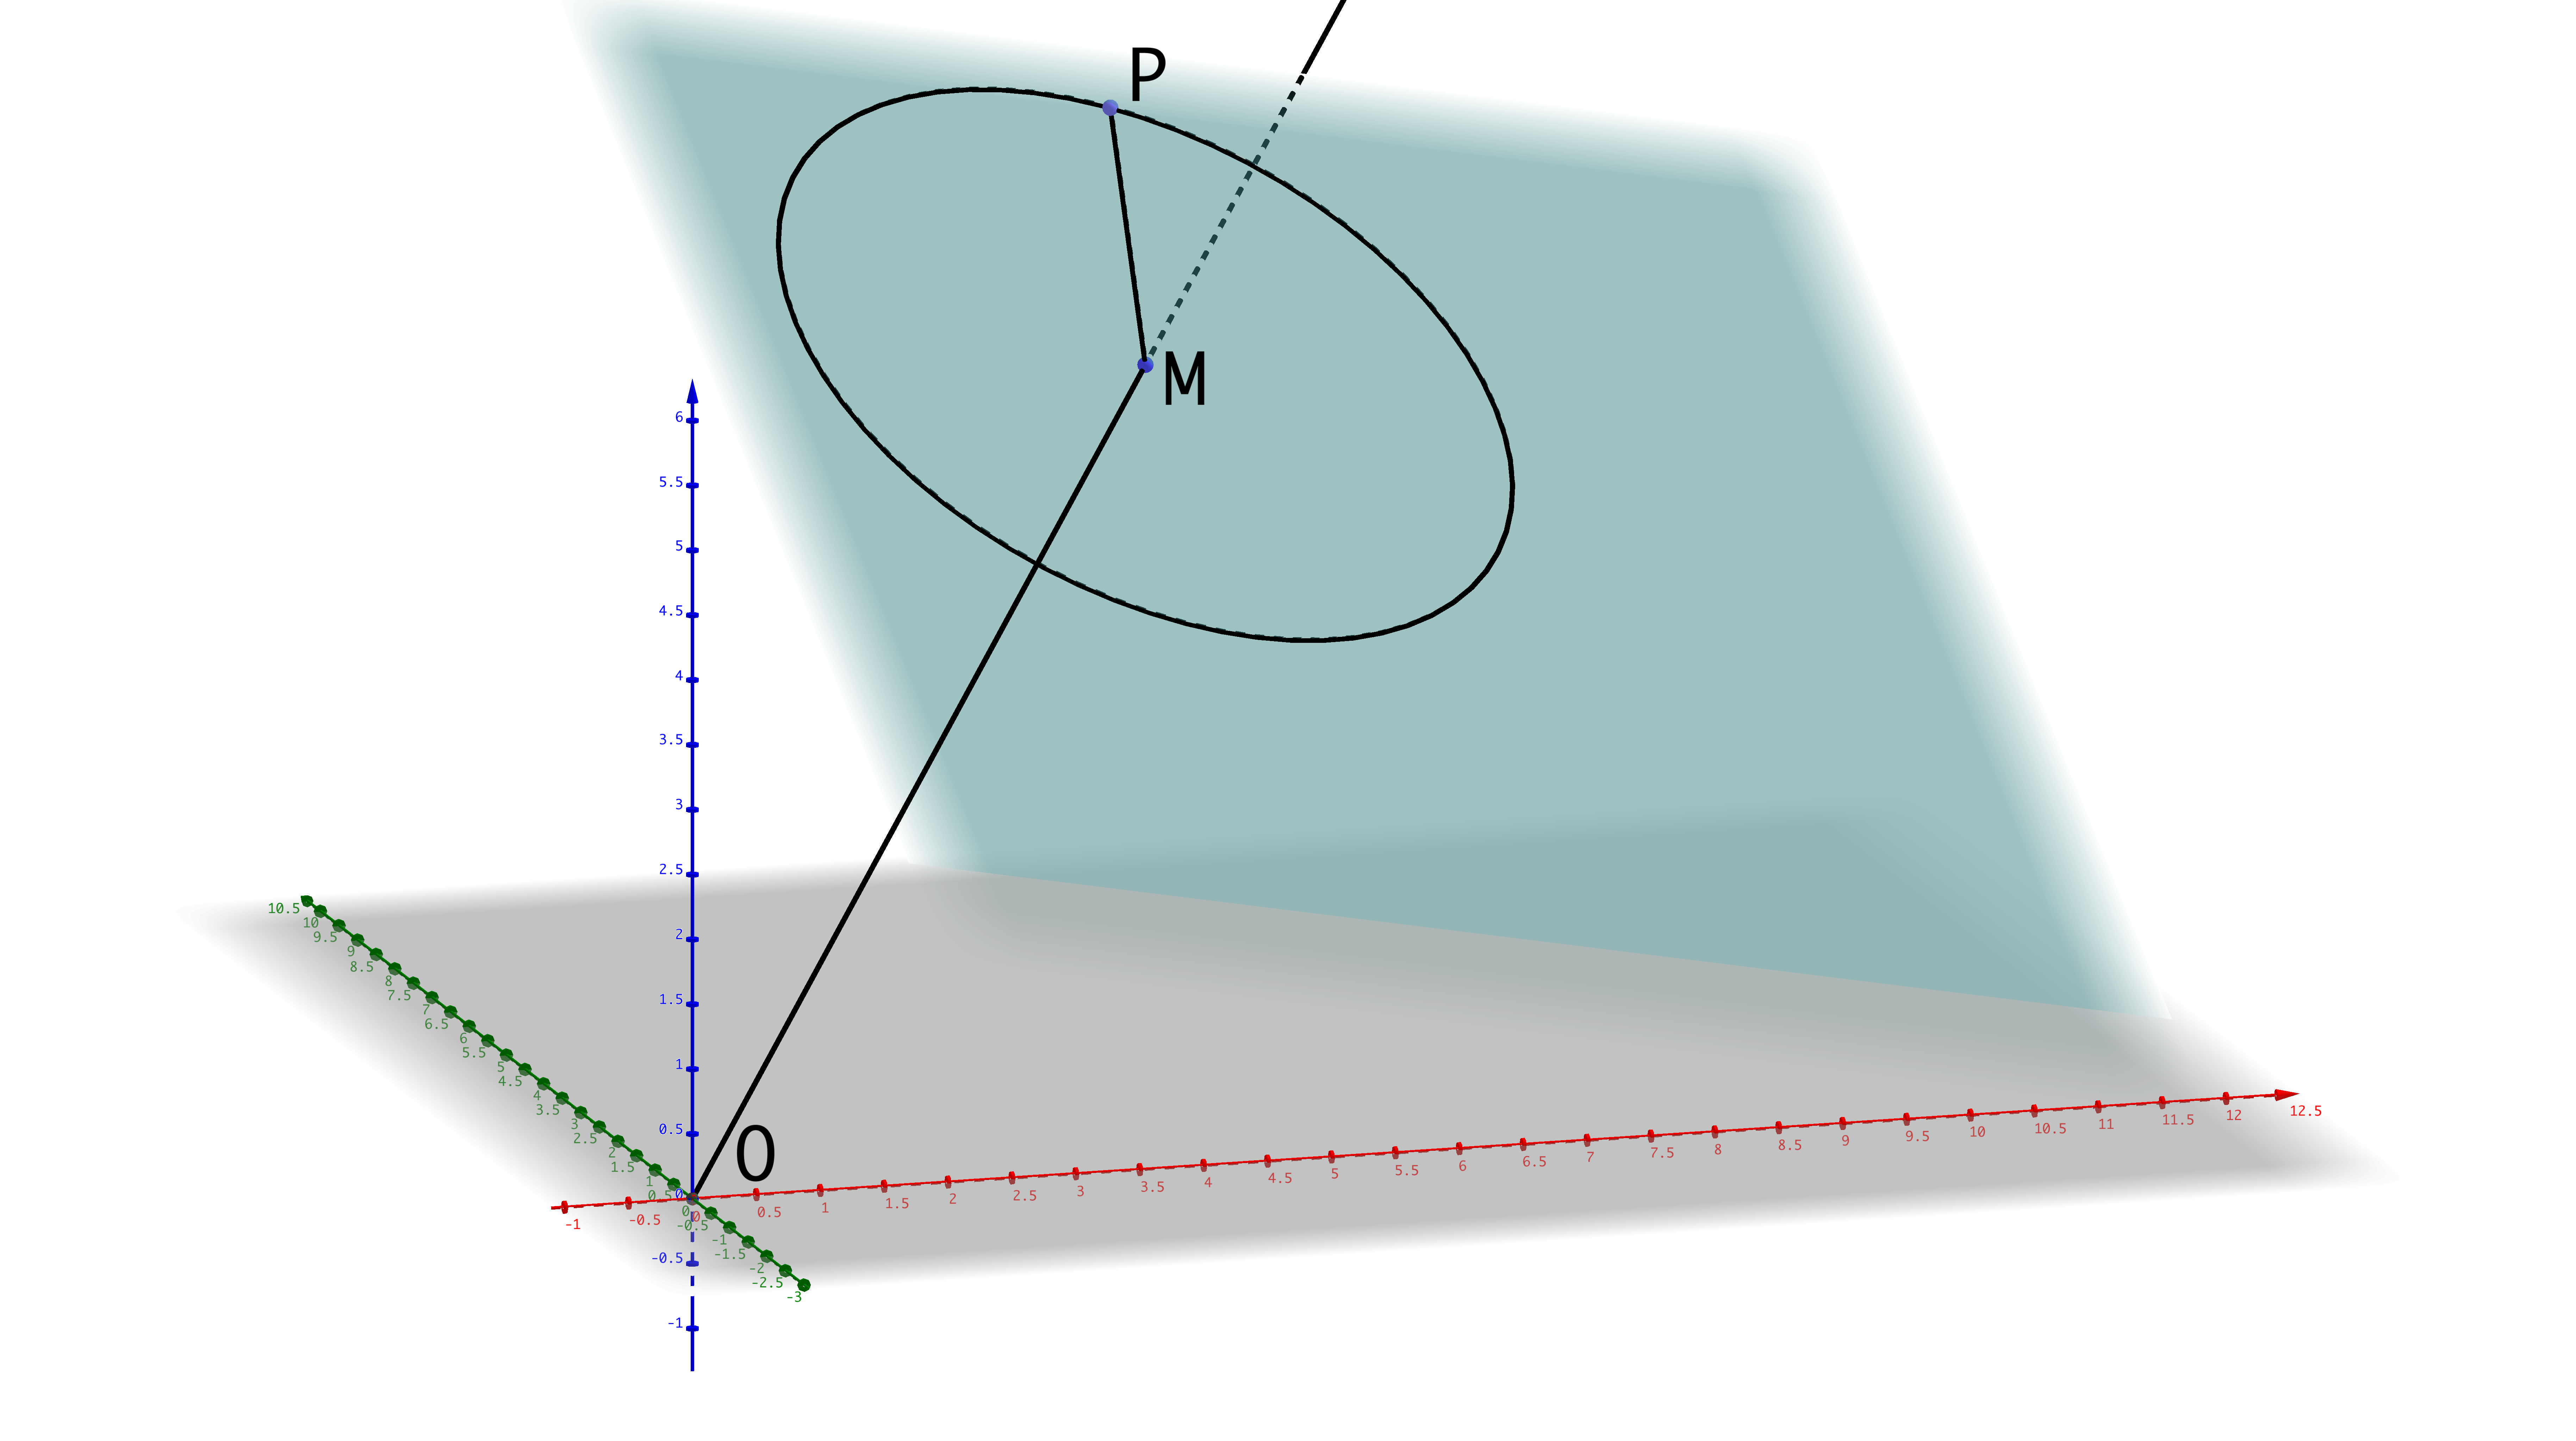
\includegraphics[width=10cm, height = 6cm]{figures/ndgeometry}
				\caption{一个三维空间中的例子}
			\end{figure}
	
			
			注意到 $OM$ 和 $P$ 所在超平面正交, 所以$\Delta \xi$ 和 $\Delta \eta$ 的变化是相互独立的. 它们对于体积的贡献也是独立的. 于是, 集合 \ref{ndgeometry} 所在的体积元体积为:
			
			\begin{equation}
				c \eta_0^{n-2} \Delta \xi_0 \Delta \eta_0
			\end{equation}
			其中 $c$ 是一个常数. 
			
			而样本的密度在这个体积元中几乎是一个常数, 为:
			
			\begin{equation}
				\begin{aligned}[]
					c \cdot \exp\left(- \frac{1}{2\sigma^2} \sum_{i=1}^n x_i^2\right) & =
					c \cdot \exp\left(- \frac{1}{2\sigma^2}(n\bar{x}^2 + \sum_{i=1}^n(x_i -\bar{x})^2)\right) \\
					& = c \cdot \exp\left(-\frac{1}{2\sigma^2} \xi_0^2\right) \cdot \exp\left(-\frac{1}{2\sigma^2} \eta_0^2\right)
				\end{aligned}
			\end{equation}
			
			这个式子和上面的体积元的表达式结合起来, 我们就可以得到元概率的表达式:
			
			\begin{equation}
				c \cdot \exp \left(-\frac{1}{2\sigma^2} \xi_0^2\right) \Delta \xi_0 \cdot \eta_0^{n-2} \exp\left(-\frac{1}{2\sigma^2} \eta_0^2\right) \Delta \eta_0
			\end{equation}
			
			这一举证明了 $\bar{x}$ 和 $s$ 的独立性.
			
			这个是一个比较有趣的地方, 对于 $t$ 分布的推导我们只有这个部分没有学习. 根据前文所述的证明梗概, 读者可以自行还原出 $t$ 分布的证明出来.